\section{Why PID is so generally applicable}
\subsection{}

\begin{frame}
\frametitleTC{The second-order process case}
\framesubtitleTC{aka ``one size fits many''}
\myPause
 \begin{itemize}[<+-| alert@+>]
 \item We consider an asymptotically  process with two poles and one zero at most, i.e.,
       \begin{displaymath}
        P(z) = \mu \frac{z-z_1}{(z-p_1)(z-p_2)}, \qquad |p_{1,2}|<1.
       \end{displaymath}
 \item We want to show that this gives rise to the four possible cases
       \begin{displaymath}
        \begin{array}{rcll}
         P_1(z) &=& \frac{\mu}{z-p_1},                                               \\
         P_2(z) &=& \frac{\mu}{(z-p_1)(z-p_2)},                                      \\
         P_3(z) &=& \frac{\mu(z-z_1)}{(z-p_1)(z-p_2)}, & |z_1|<1,                    \\
         P_4(z) &=& \frac{\mu(z-z_1)}{(z-p_1)(z-p_2)}, & |z_1|>1 \text{ or } z_1=-1, \\
        \end{array}
       \end{displaymath}
       and that each of these is very naturally paired to a PI(D) controller.
 \item But: why not a case with one pole and one zero? Why not $z_1=1$?
 \item We need another short \emph{intermezzo}...
 \end{itemize}
\end{frame}

\begin{frame}
\frametitleTC{Why not $z_1=1$}
\framesubtitleTC{}
\myPause
 \begin{itemize}[<+-| alert@+>]
 \item We start from the simple. If $z_1=1$ the process output $y$ tends asymptotically to zero
       for any constant input $u$, as it comes to depend on $u(k)-u(k-1)$.
 \item This means that to keep $y$ at a certain constant reference value, $u$ should indefinitely
       increase at a corresponding constant \TC{rate}, up to infinity---or overflow.
       Apparently, such a process cannot be managed (control people use to say ``you cannot prescribe
       the steady state'').
 \item If conversely $z_1=-1$ one can prescribe the steady state, but not cancel the zero with a
       pole of $C$, or the cancellation would be critical, as we already know.
 \item We thus consider $z_1=-1$ and $|z_1|>1$ the same case, and we know\\
       what the outcome will be.
 \item More interesting is to discuss why we assume $P$ to be always strictly\\
       proper (more poles than zeroes). 
 \end{itemize}
\end{frame}

\begin{frame}
\frametitleTC{A controller's execution timeline}
\framesubtitleTC{Some considerations}
\myPause
 \begin{itemize}[<+-| alert@+>]
 \item Let us first point a further peculiarity of control in computers.
       \begin{itemize}[<+-| alert@+>]
       \item When the controlled object is outside the computer, it always evolves in \TC{physical}
             parallel with the controller's execution; when it is inside, that parallel might be physical
             or just emulated, if the two entities share a CPU. Said otherwise, \TC{running the controller
             can halt the process}.
       \item More in general, in non-computer applications, running controllers adds value to the process
             by improving its operation. In computers, on the contrary, time to compute the control signals
             is \TC{anyway stolen} from that devoted to applications. And since value ultimately comes from
             running applications, time for running controllers must be almost negligible.
       \end{itemize}
 \item For the sake of completeness, the second statement may not hold\\
       if the control payback is really huge, or if controllers have dedicated\\
       hardware to run; we leave discussing such cases to advanced\\
       activities, however.
 \end{itemize}
\end{frame}

\begin{frame}
\frametitleTC{A controller's execution timeline}
\framesubtitleTC{Some considerations}
\myPause
 \begin{itemize}[<+-| alert@+>]
 \item In general -- i.e., considering also cases we do not address in our activity -- one can distinguish
       three cases (thinking for simplicity of a sampled signals context):
       \begin{itemize}[<+-| alert@+>]
       \item the time $\tau(k)$ to compute the generic $u(k)$ is negligible wrt the sampling period $T_s$;
       \item $\tau(k)$ is not negligible wrt $T_s$ but it is -- almost -- invariant (no branches, no operations
             with operand-dependent duration, no or negligible cache effects, and so on---or countermeasures taken
             in the code for such issues);
       \item $\tau(k)$ is not negligible wrt $T_s$ and can vary significantly over the control steps.
       \end{itemize}
 \item We do not have the time to investigate the matter (but those who want to deal\\
       safely with high-performance real-time control \TC{should} study it very\\
       carefully in control technology courses).
 \item In fact a PI(D) algorithm can be made very lightweight (down to a\\
       few tens of clock cycles, to give a figure) so that we are practically\\
       always in the first case.
 \end{itemize}
\end{frame}

\begin{frame}
\frametitleTC{A controller's execution timeline}
\framesubtitleTC{Some considerations}
\myPause
 \begin{itemize}[<+-| alert@+>]
 \item The timeline is therefore as follows:
       \begin{center}
        \vspace{1mm}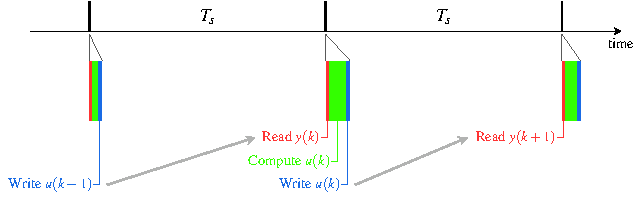
\includegraphics[width=0.70\columnwidth]{./Unit-07/img/CtrlTimeline.pdf}
       \end{center}
 \item As can be seen, the effect of $u(k)$ can be seen only at step $k+1$,\\
       hence the process is correctly viewed as a strictly proper model.
 \item Incidentally, being in the first case is essential to make the P action\\
       possible.
 \item ...end of the \emph{intermezzo}.
 \end{itemize}
\end{frame}

\begin{frame}
\frametitleTC{Back to the second-order process}
\framesubtitleTC{for a reasoned recap and a systematisation}
\myPause
 \begin{itemize}[<+-| alert@+>]
 \item Exercise: take the four cases
       \begin{displaymath}
        \begin{array}{rcll}
         P_1(z) &=& \frac{\mu}{z-p_1},                                               \\
         P_2(z) &=& \frac{\mu}{(z-p_1)(z-p_2)},                                      \\
         P_3(z) &=& \frac{\mu(z-z_1)}{(z-p_1)(z-p_2)}, & |z_1|<1,                    \\
         P_4(z) &=& \frac{\mu(z-z_1)}{(z-p_1)(z-p_2)}, & |z_1|>1 \text{ or } z_1=-1. \\
        \end{array}
       \end{displaymath}
 \item For each of them select a controller structure, devise a way to provide\\
       a response speed specification, and formalise a tuning procedure;\\
       then build a Modelica LTI scheme to simulate the so obtained\\
       loops, design and carry out experiments, and comment.
 \end{itemize}
\end{frame}

